\documentclass[]{article}
\usepackage{graphicx}
\usepackage{enumitem}


\title{Architecture Report}
\author{KTH Group 2} % Please don't add names!

\begin{document}

\maketitle

\section*{Component Overview}
The different components of the system can be found in
Figure~\ref{fig:system_diagram}, where there are three principal
components:
\begin{enumerate}
\item Workload generator
\item Service
\item Monitor
\end{enumerate}

\begin{figure}[!t]
  \centering
  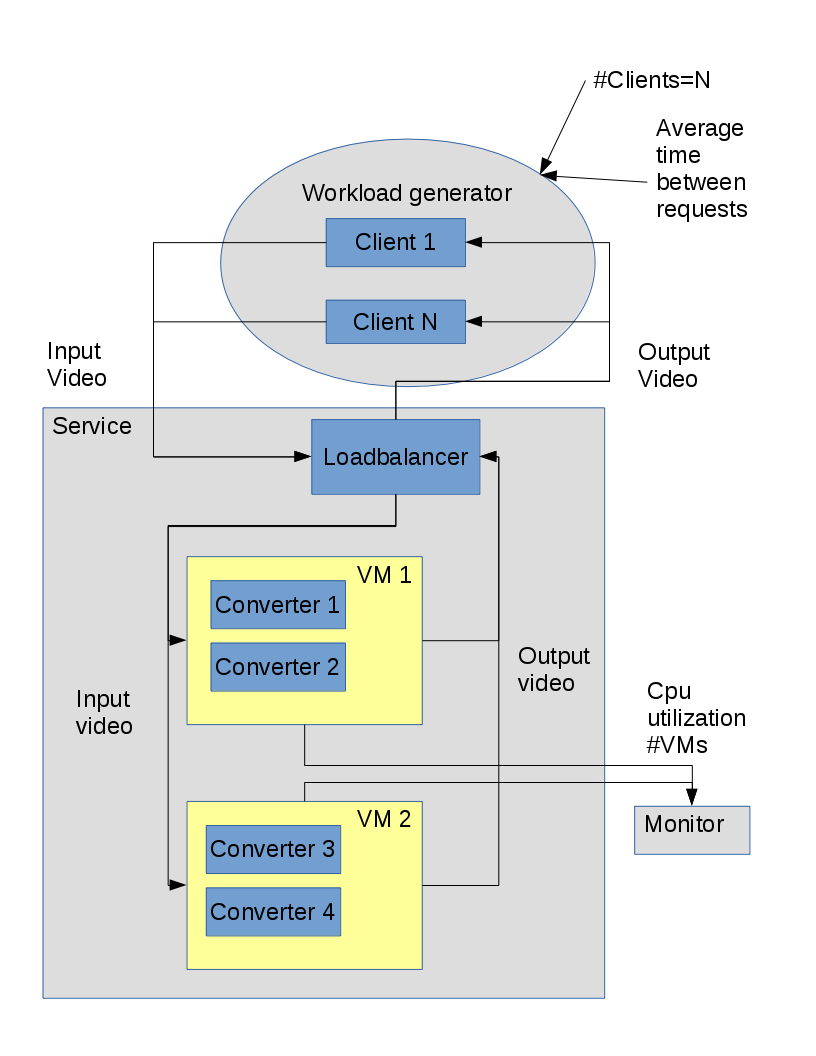
\includegraphics[width=\linewidth]{system_diagram}
  \caption{Graphical representation of the requirements and the
    components.}
  \label{fig:system_diagram}
\end{figure}

\section*{Architecture of the Application}

\begin{figure}[!t]
  \centering
  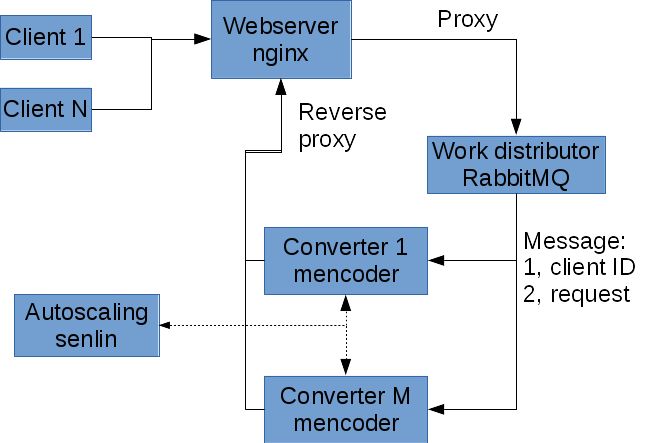
\includegraphics[width=\linewidth]{arch_diagram}
  \caption{Architecture of a video converting application.}
  \label{fig:arch_diagram}
\end{figure}

A schematic representation of the architecture can be found in
Figure~\ref{fig:arch_diagram}. The clients connect to the webserver,
which is a nginx webserver, and the webserver produces a job message which it
puts in the distributed queue, RabbitMQ. A job message consists of:
\begin{enumerate}
\item Client ID, for the webserver to identify the client.
\item Additional information about the request.
\end{enumerate}
A VM consumes a message from the queue, and sends a confirmation
message to the client, via the webserver acting as a reverse proxy
server now. The client gets the confirmation and an URI to where the
client can use the HTTP POST command to send his input video. 
The converter gets the input video, process the video, and
sends it back to the client, via the webserver. This process is
depicted in Figure~\ref{fig:sequence_diagram} shows the sequence
diagram, which consists of the following messages:
\begin{enumerate}
\item The client requests a video conversion from the frontend.
\item The frontend requests the necesary resources from the backend.
\item The backend reserves the necessary resources.
\item The backend acknowledges by providing a resource block.
\item The frontend acknowledges that the video can be converted.
\item The client can start transferring the source video.
\item The backend converts the video to the desired format.
\item The resulting video file is transfered back to the client.
\end{enumerate}

\begin{figure}[h]
  \centering
  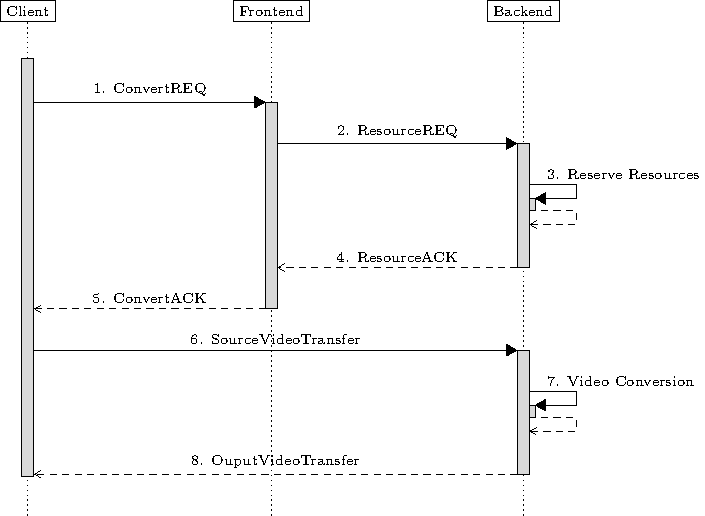
\includegraphics[width=\linewidth]{sequence_diagram}
  \caption{}
  \label{fig:sequence_diagram}
\end{figure}

The OpenStack Senlin module surveys and monitors the load on the
converter nodes. Senlin can use different policies to scale up and
down the number of running vm. The senlin module would also act as the
monitor in the component scheme.

The architecture have the following properties:
\begin{itemize}
\item No files are stored in the service.
\item The requests are relayed from the webserver to the work distributor, a distributed message queue.
\item A job consists of three parts:
  \begin{enumerate}
  \item Send the video from the client to the worker, through proxy server.
  \item The worker process the video.
  \item The worker sends back the converted video to the client, through proxy server
  \end{enumerate}
\item The senlin module scales the number of running VMs, based on predefined policies.
\end{itemize}

\section*{Exposed Interfaces}

The following interfaces are implemented:

\begin{enumerate}
\item REST HTTP API between client and webserver.
\item HTTP XML between nginx distributed queue (STOMP).
\item Openstack between converter VM and senlin.
\end{enumerate}

\section*{Technology Stack}
\begin{enumerate}
\item PyFLASK
\item Pyrequest
\item nginx
\item RabbitMQ
\item Senlin
\item mencoder
\item Python wrapper for mencoder
\end{enumerate}

\section*{Scalability and Robustness}

\begin{itemize}
\item Three vms are assumed to be always-available:
  \begin{enumerate}
  \item webserver
  \item work distributor
  \item autoscaling
  \end{enumerate}
\item The converter node VMs can be scaled up or down depending on the need.
\end{itemize}


\end{document}

%%% Local Variables:
%%% mode: latex
%%% TeX-master: t
%%% End:
